Il numero della popolazione che utilizza Internet è in grande crescita, grazie all’ampia diffusione di dispositivi mobili e alla maggiore disponibilità di accesso alla rete. Tutto questo sta influenzando, sempre più, anche il sistema economico. Sul Web da una parte ci sono i consumatori che svolgono le loro attività quali: ricerca dell’informazione, feedback, condivisione materiale multimediale (immagini, video, etc.) e partecipazione alle community, etc.. Dall’altra ci sono le aziende per le quali, Internet, rappresenta un mezzo di comunicazione molto efficace per apparire sul mercato e presentare i propri prodotti e/o servizi. In particolare, attraverso il Web, le aziende sono in grado di offrire promozioni, offerte, ed assistenza personalizzata, grazie alla profilazione dell’utente che avviene rapidamente.
\newline
Quando Internet iniziò a diventare un fenomeno di massa, le aziende ne hanno subito captato le potenzialità comunicative e l’opportunità per farsi conoscere, per raccontare la propria storia e per mostrare il loro output produttivo e così entrare nel mercato internazionale.
\newline
Per ottenere una maggiore visibilità e essere più competitiva sul mercato globale l’azienda deve quindi adottare il nuovo canale di vendita: l’e-commerce (commercio elettronico).
\begin{figure}[htb]
 \centering
 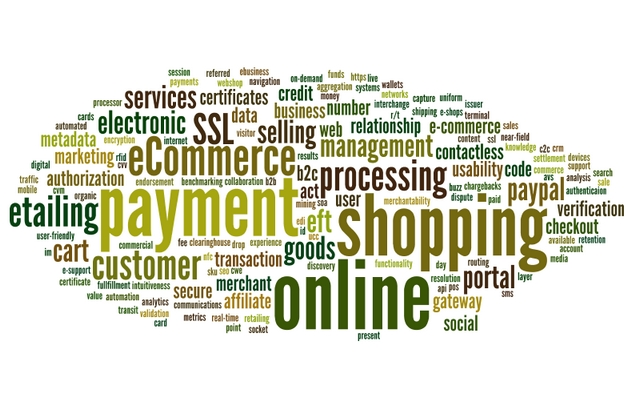
\includegraphics[width=1.0\linewidth]{images/introduction/ecommerce-wordle.jpg}\hfill
 \caption[e-commerce wordle]{e-commerce wordle}
 \label{fig:e_commerce_wordle}
\end{figure}
Nel 1970, il termine “e-commerce” si riferiva a scambio elettronico di dati per l’invio dei documenti aziendali come gli ordini di acquisto. Successivamente, grazie allo sviluppo tecnologico, il commercio elettronico è diventato un’attività di scambio di beni e servizi attraverso il Web \cite{commerce_intro_1}, permettendo di consolidare l’abitudine ad acquistare on-line da parte dei clienti, che hanno, così aumentato la quota di spesa on-line sul consumo totale.
\newline
L'esistenza di questi negozi virtuali, che non occupano spazio fisico (quindi abbattono costi fissi di gestione), permettono di accedere al negozio 24 ore su 24 da qualsiasi parte del mondo, oltre ad offrire una gamma di prodotti (inseriti nelle vetrine virtuali) che facilitano il consumatore nella scelta risparmiando così del tempo.
\newline
Grazie a tutte queste opzioni, il commercio elettronico è considerato il “miracolo” del nostro secolo.
\newline
E' dunque il Web, il primo canale per le aziende che permette loro di affermarsi sul mercato e aumentare il proprio profitto.
Tale processo, innanzitutto, inizia con la creazione di un proprio sito istituzionale, un vero e proprio “biglietto da visita”, per mostrarsi al mondo digitale. Considerando che, è molto importante per un’azienda apparire sul mercato il prima possibile rispetto alle sue concorrenti, la creazione di un proprio portale deve avvenire in tempi non troppo lunghi e deve essere di facile costruzione.
\newline
Per tale scopo esistono diverse piattaforme che facilitano la realizzazione di un sito personale che permette di vendere prodotti o servizi. Queste piattaforme offrono diversi servizi per facilitare il più possibile il venditore come: gestione dell’inventario, inserimento - cancellazione - modifica di prodotti, creazione di collezione di prodotti, uno o più servizi di pagamento, spedizione/tracking, etc.. Il tutto attraverso un’interfaccia di facile utilizzo in maniera tale che, chiunque possa usufruirne.
\newline
Shopify, Bigcommerce, Prestashop, 3dcart, WIX.com, etc. sono piattaforme che offrono questi tipi di servizi. Questi sistemi se da una parte hanno una struttura ben consolidata, spesso sono poco flessibili per via del fatto che esistono da diversi anni e risultato pertanto sviluppati con tecnologie che oggi sono superate.


Il lavoro svolto in questo progetto di tesi ha come obiettivo la realizzazione di una piattaforma, X-commerce, in grado di competere con queste grandi compagnie, attraverso nuove tecnologie.

Oltre a mettere a disposizione le stesse funzionalità su cui si basano le piattaforme già esistenti, si vuole offrire un modo più efficace e flessibile per integrare nuovi servizi, che fin'ora sono stati difficile da realizzare.

% cosa che le altre piattaforme riescono a realizzare con diverse difficoltà.


\newline
X-commerce mira ad offrire agli sviluppatori un nuovo metodo, basato su componenti riutilizzabili, per comporre le proprie pagine web (orientati all’e-commerce).
\newline
X-commerce utilizza una tecnologia recente di Google chiamata Polymer, che implementa lo standard dei Web Components, la cui caratteristica principali è la riusabilità del codice.
\newline
Come detto dagli autori di Polymer-Project: “Tutto è un elemento, anche un servizio ” \cite{polymer_world_view}. Questa è la filosofia che X-commerce segue, per cui ogni tipo di funzione o responsabilità è incapsulata in elementi Polymer diversi ed auto-contenuti. Dunque X-commerce ha l’obiettivo di voler semplificare la vita agli sviluppatori di applicazioni web (orientati all’e-commerce) nella realizzazione di pagine web che avviene assemblando diversi componenti.
\newline
Questa tesi è divisa in due parti ed è organizzata come segue:
\begin{itemize}
\item
la prima parte si compone di tre capitoli: il primo descrive lo stato dell’arte sulle piattaforme che facilitano la realizzazione di sistemi e-commerce come Shopify, Bigcommerce, etc.; il secondo descrive le tecnologie abilitanti per i servizi di pagamento che non possono mancare in un sistema di e-commerce ed il terzo mostra una panoramica generale sulle principali tecnologie utilizzate per realizzare X-commerce come Polymer, Loopback, etc.
\item la seconda parte si compone di altri tre capitoli: il quarto descrive l'architettura di X-commerce e mette in luce i principali schemi e modelli dello stesso; il quinto si focalizza principalmente su un componente specifico ovvero la gestione dei pagamenti, servizio indispensabile per un sistema di e-commerce mentre il sesto ed ultimo espone le conclusioni tratte e fornisce dei possibili sviluppi futuri per il progetto.
\end{itemize}